\documentclass{article}

\usepackage{geometry}
\usepackage{hyperref}
\usepackage{graphicx}
\usepackage{float}
\usepackage{cite}
\title {CS 201: Data Structures II \\Merkle Trees} % Mention your project title

\author{Group 3} % Mention your team name
\date{Spring 2023}  

\begin{document}
\maketitle
\section{Group Members}
% Mention your Group Members and their ids
\begin{enumerate}
  \item Muzzammil Sattar ms07164
  \item Arsalan Hussain mh07607
  \item Abdullah Junejo aj07154
  \item Anas Bin Yousuf ab07351
\end{enumerate}
\section{Data Structure}
We will create a localized implementation of block-chain using Merkle trees and a simple Linked List. 
Merkle trees will be used to encrypt the data using a collision resistant hash function. 
\section{Application}
We will demonstrate encryption and security of documents by using our own block chain. We will further show how a Merkle Tree effectively identifies if any given document has been changed or corrupted.  
\section{Functionality}
The Merkle Tree has two key functions: 
\\\\
1) Encryption: This is where the Merkle Tree (or Block) is created using the decided data/documents and collision resistant hash function.
\\\\
2) Verification: This is where we use Merkle Proofs to efficiently check if a given data/document belongs to the Tree and also to verify (through hashing) if the given data/document has been altered or corrupted.
\\\\
We will now talk about Encryption and the creation of the Merkle Tree in a little more depth:
\\\\
To construct the Merkle Tree we start at the leaf nodes, and create layers until we reach the root node which is our root hash. 
\\\\
For example if we have 8 documents we will hash all 8 documents to produce 8 hashes, this is our zeorth layer. We will then hash each pair (Document 1's hash with Document 2's, Document 3's hash with Document 4's, Document 5's hash with Document 6's). This will result in 4 hashes that make up the first layer. Pairs of these four hashes are then hashed together to form the second layer consisting of two hashes, which are then hashes together to form the root hash. The image below illustrates this:

\begin{figure}[htp]
    \centering
    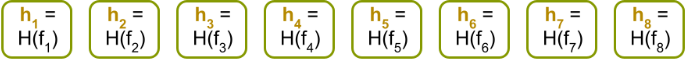
\includegraphics[width=12cm]{Layer 0}
    \caption{The Zeroth Layer}
    \label{fig:f1}
\end{figure}

\begin{figure}[htp]
    \centering
    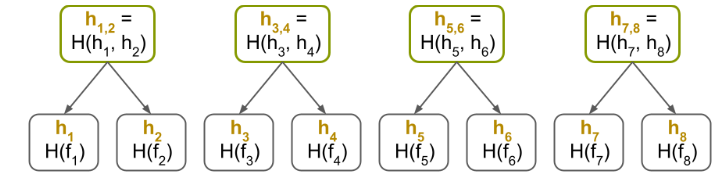
\includegraphics[width=12cm]{Layer 1}
    \caption{The First Layer}
    \label{fig:f2}
\end{figure}

\begin{figure}[htp]
    \centering
    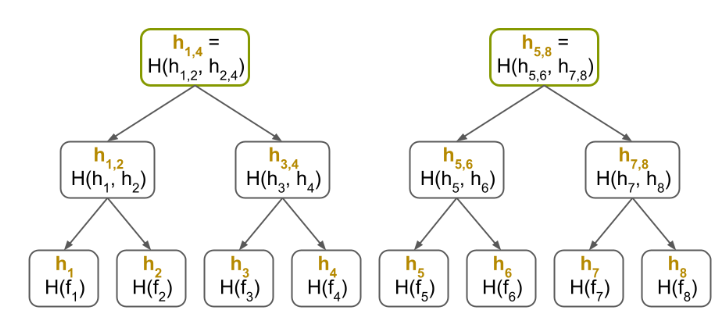
\includegraphics[width=12cm]{Layer 2}
    \caption{The Second Layer}
    \label{fig:f3}
\end{figure}

\begin{figure}[htp]
    \centering
    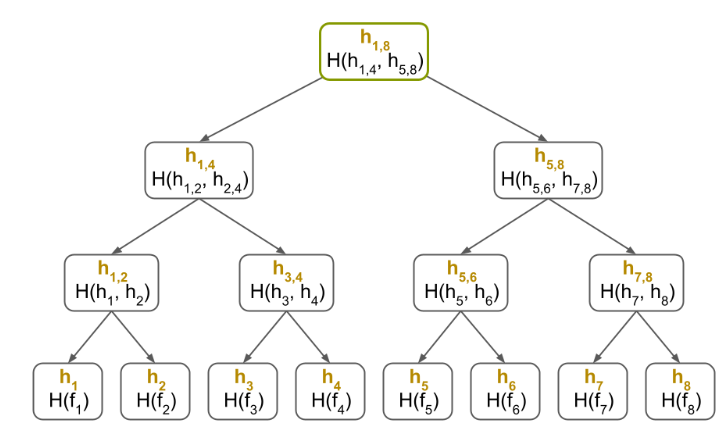
\includegraphics[width=12cm]{Final Layer}
    \caption{The Final Layer and Root Hash}
    \label{fig:f4}
\end{figure}

.
\\\\\\
This can be done for any n number of documents, where after the zeroth layer we hash the pairs to produce n/2 hashes. Those pairs are then hashed to produce n/4 hashes and so on until we reach n/n hashes which is the final layer that is the root hash.
\\\\
Once a Merkle Tree or Block has been created no other documents can be added to it. If there is a new related set of documents that need to be inserted, these documents are made into their own Merkle Tree or Block. The Blocks are then linked together using a simple Link List.
\\\\
We will now discuss the verification process:
\\\\
Merkle Tree's are efficient at verifying if a document has been changed as an altered document would produce a hash that is different from the root hash. If the document hasn't been changed then the same root hash would be produced. This is the bases of a Merkle Proof. Furthermore only a set of hashes would be needed to prove a given leaf's membership in the tree as illustrated below for the example discussed earlier:

\begin{figure}[htp]
    \centering
    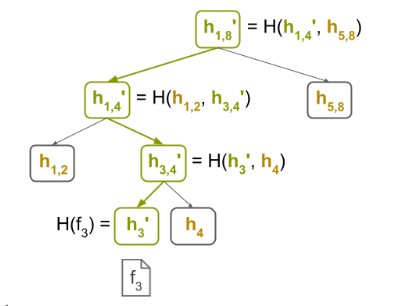
\includegraphics[width=8cm]{Merkle Proof}
    \caption{Merkle Proof}
    \label{fig:f4}
\end{figure}
.
\\\\\\\\\\
\section{Datasets}
While we have not come up with a particular dataset at this time, we plan to have our dataset related to documents. It should be noted that our dataset is one which we should be able to change or corrupt after using it to make the Merkle Tree to demonstrate its Validation Functionality.
\newpage
\section{Work Distribution}
Fill in the table which indicates the work distribution of each member.
\begin{center}
  \begin{table}[h]
    \centering
    \begin{tabular}{|c|c|c|}
      \hline
      Item & Activity   & ID      \\ \hline
      1    & Researching and Exploring the functionality of Merkle Tree's (Verification and Encryption) & mh07607 \\ \hline
      2    & Writing this Documentation and Researching the process of Verification and Encryption & ms07164 \\ \hline
      3    & Exploring the application and looking at sample code & ab07351 \\ \hline
      4    & Exploring the application and looking at sample code & aj07154 \\ \hline
    \end{tabular}

    \label{tab:my-table6}
  \end{table}
\end{center}
\section{Attribution}

\begin{thebibliography}{9}
https://decentralizedthoughts.github.io/2020-12-22-what-is-a-merkle-tree/
https://www.geeksforgeeks.org/introduction-to-merkle-tree/
  \end{thebibliography}
\end{document}

